\section*{Zielsetzung}
Die Zielsetzung dieses Versuchs ist es die Funktionsweise eines He-Ne-Lasers kennenzulernen. Dazu werden verschiedene Eigenschaften des Laserlichts, wie die Wellenlänge, die Intensitätsverteilung, die Polarisation, das Modenspektrum und der Einfluss der Resonatorlänge auf die Stabilität des Lasers untersucht.

\section{Theorie}
\label{sec:Theorie}

Die Abkürzung Laser steht für den Begriff \textit{"Light Amplification by Stimulated Emission of Radiation"}.
Ein Laser besteht aus drei Hauptkomponenten, die es ermöglichen einen Laserstrahl zu erzeugen. Diese sind ein aktives Lasermedium, eine Energiepumpe und ein Resonator.
\newline
Im \textbf{aktiven Lasermedium} finden die Übergänge zwischen unterschiedlichen Energieniveaus statt. Beim He-Ne-Laser ist das Neon das aktive Lasermedium, in dem die zentralen Prozesse Absorption, spontane Emission und stimulierte Emission stattfinden. Diese Prozesse sind in \autoref{fig:emission} schematisch dargestellt. Der entscheidende Prozess bei einem Laser ist die stimulierte Emission, da hier das ausgesendete Photon die gleiche Bewegungsrichtung wie das eingestrahlte Photon hat.

\begin{figure}[H]
  \centering
  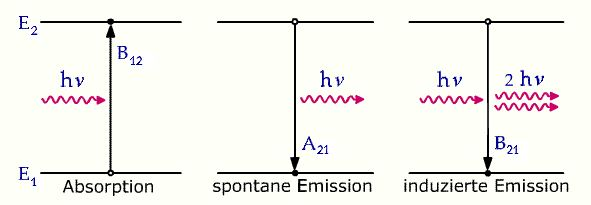
\includegraphics[width=1\textwidth]{images/emission.JPG}
  \caption{Schematische Darstellung der möglichen Strahlungsübergänge. \cite{emission}}
  \label{fig:emission}
\end{figure}

\noindent
Die \textbf{Energiepumpe} beim He-Ne-Laser ist das Heliumgas, welches zuerst durch Anlegen einer Spannung energetisch angeregt werden muss. Die He-Atome stoßen mit Ne-Atomen zusammen und bringen diese in einen angeregten Zustand. Dadurch werden die Ne-Atome zur Besetzungsinversion angeregt, was heißt, dass sich mehr Elektronen in einem energetisch höheren als in einem energetisch niedrigeren Niveau befinden. Das Energieniveauschema für den He-Ne-Laser ist in \autoref{fig:laser} dargestellt.
\begin{figure}[H]
  \centering
  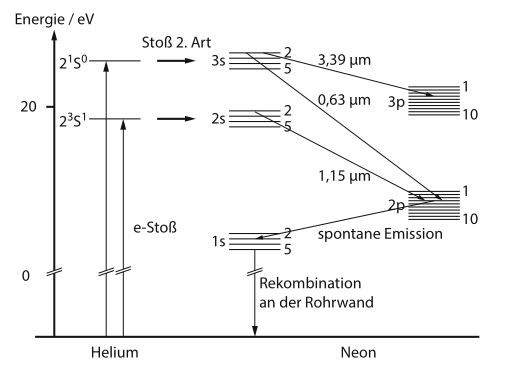
\includegraphics[width=1\textwidth]{images/niveaus.JPG}
  \caption{Energieniveauschema des He-Ne-Lasers. \cite{laser}}
  \label{fig:laser}
\end{figure}
\noindent
Es ist also zu erkennen, dass die betrachtete rote Laserlinie bei $\lambda = \SI{630}{\nano\metre}$ durch den Energieübergang von 3s zu 2p entsteht.
\newline
\noindent
Der \textbf{Resonator} ist eine Anordnung aus zwei sich gegenüber stehenden Spiegeln, welche dazu dient das Laserlicht durch wiederholte stimulierte Emission zu verstärken. Außerdem legt der Resonator durch seine Anordnung die Richtung der stimulierten Emission fest. Wenn die Verluste in einem Resonator geringer sind als die Verstärkung durch die stimulierte Emission, gilt dieser als stabil. Dies wird mathematisch durch die Stabilitätsbedingung

\begin{equation}
    0 \leq g_1 \cdot g_2 < 1
    \label{eqn:Stabilität}
\end{equation}
\noindent
beschrieben. Mit der Resonatorlänge $L$ und den Krümmungsradien $r_i$ sind die Stabilitätsparameter $g_i$ durch die Formel
\begin{equation}
    g_i = 1 - \frac{L}{r_i}
\end{equation}
\noindent
gegeben.
\newline

\noindent
In einem solchen Resonator können sich stehende Wellen ausbilden, die man als TEM-Moden bezeichnet. Dabei werden longitudinale und transversale TEM-Moden unterschieden. Die $TEM_{00}$-Mode ist die Grundmode, deren Intensität die Form einer Gaußkurve nach 
\begin{equation}
  I(r) = I_0 \exp{\frac{-2 \, r^2}{w^2}}
  \label{eqn:gauss}
\end{equation}
\noindent
aufweist. Moden höherer Ordnung werden Multimoden genannt und weisen in der Regel eine unregelmäßigere Lichtintensität auf. Daher liefern höhere Moden Laserstrahlen von schlechterer Qualität.
